\section{Runtime System Overview}


Briefly, the runtime system we are building will execute dataflow applications
with dependency among stages, utilizing distributed CPU-GPU equipped platforms.
The overall execution model is based on a bag of tasks, where tasks are
instantiations of a given stage of the application dataflow --- the pair input
data and stage processing functions. To guarantee correct ordering in the
execution of such tasks, the runtime system will use task dependency
information given as input by the user through a simple API, and will assert
that a tasks is not dispatched for execution before all dependencies are
solved. 


%\subsection{Overview}


\begin{figure}[ht]
\begin{center}
\includegraphics[width=0.47\textwidth]{images/appDataflow}
\caption{Sample Application Dataflow.}
\label{fig:sampleDataflow}
\end{center}
\end{figure}

Further, communication among the pipeline stages, or tasks, is performed
through a distributed file system, meaning that data is read and written to
files between stages. Figure~\ref{fig:sampleDataflow} presents a schema of the
multiple levels that may be used to represent a dataflow in this model. In the
first level, Abstract Dataflow, we simply have the logical stages of the
application, describing their connections. In the second level, there is the
instantiation of the dataflow, where the logical computing stages are
associated to different input data, and dependencies among instantiation of
stages (Tasks) are described. For instance, in the left side, there is an
instantiation of the dataflow with an independent replication of the entire
pipeline for each input data.  In the right side, however, there is a more
complex interaction in the dataflow as each input data is computed in parallel
in through multiple instantiations of first stage, but the following stages on
the pipeline will use results computed from the previous instantiations of
stage A (A.1 and A.2). On the bottom level of the same figure, we show that
each logical stage of the application may again be another pipeline, with
dependencies among sub-stages that may additionally have implementation for
multiple devices, e.g. CPU or/and GPU. 

Providing a stage with the capabilities of being described as a pipeline of
multiple sub-tasks has to be (i) with the need of exporting operations with
different performance to the local scheduler (described latter, but similar to
IPDPS), and (ii) with necessity of providing an efficient way for the
application to execute a number of sub-stages without having to write the
output of each of them to the file system, as is necessary in the
communication among stages of the application pipeline.



\begin{figure}[ht]
\begin{center}
\includegraphics[width=0.47\textwidth]{images/executionModel}
\caption{Overview of the system architecture, and task mapping.}
\label{fig:execModel}
\end{center}
\end{figure}

Figure~\ref{fig:execModel} shows the runtime system design, with an overview of
the interaction among its components. In this system, the \emph{Manager} is the
process responsible for handling dependencies among different instantiations of
the dataflow stages (Tasks) (middle level of Figure~\ref{fig:sampleDataflow}),
and to dispatch those tasks for execution with the \emph{Workers}. The
\emph{Workers} will communicate with the \emph{Manager} to request tasks to
compute, retrieve those tasks, and executed them. Each task will read data from
a file system and may spawn a pipeline of sub-tasks that is locally scheduled
by each \emph{Worker}.  When all sub-tasks of a given task are computed, the
\emph{Worker} informs the \emph{Manager}, which may assign another task for
execution. In practice, a single worker may execute multiple Stages, even
concurrently, and both sets of workers presented in Figure~\ref{fig:execModel}
are not necessarily disjoint. 


\begin{figure}[ht]
\begin{center}
\includegraphics[width=0.47\textwidth]{images/worker-environment}
\caption{Workers Environment: the workers is a multi-thread process that may
take advantage of all processing elements in a node to execute the
applications' tasks.}
\label{fig:workerEnv}
\end{center}
\end{figure}

The environment of each Worker, shown in Figure~\ref{fig:workerEnv}, is similar
to what we proposed for IPDPS, with addition of a few features. As discussed,
task dependency management has been added, as well as the communication layer
module that is coupled to abstract exchange of information with the
\emph{Manager}.




